\chapter{Using Stellar Command with OSC} \label{chap:launchosc}
There are primarily two ways to use Stellar Command. The first is as a separate process that runs on the compute. The second method is to use Stellar Command as a library that you link to directly in your program. If you intend to use Stellar Command as a library, you can skip forward to chapter~\ref{chap:libraryosc} --
\emph{\titleref{chap:libraryosc}}.


\section{Launching Stellar Command}
makeidx{standalone}
\index{osc!clientport}
\index{osc!port|}
The Stellar Command module is instantiated by executing Java  with the name of the JAR file and the required program arguments that define communication, such as the network port to send OSC messages to, and the OSC address space.  For example, to start the StellarCommand module so it sends OSC messages on UDP port 1234  using an OSC address space of \texttt{/Stellar},\footnote{In this instance, the OSC client and Stellarium are on the same computer.} one would execute the following command:\\

\begin{syntax}

	java -jar StellarCommand.jar port=1234 osc=/Stellar  \\

\end{syntax}
\bigskip
   When the server starts, it will open the first available UDP port, and notify the client of this port. For example, if the command module opened port 4567, it will send an OSC message \texttt{/Stellar/osc 4567} to the client on the localhost. 
   
\begin{syntax}

	/Stellar/osc 4567  \\

\end{syntax}
\bigskip

Allowing the command module to find its own port number removes the probability of port clashes as each client furnishes the other with a valid port number for communicating without requiring configuration in the command module. It is, however, possible to request the Stellar Command module try certain ports by adding the argument \textit{tryport} \index{osc!tryport|(} with a comma separated list of ports. For example, the argument \texttt{tryport=3333,4444,5555} will cause Stellarium to sequentially try opening the ports listed, and if these all fail, will then open the first available port.\\
   
   \begin{syntax}

   	java -jar StellarCommand.jar port=1234 osc=/Stellar  tryport=3333,4444,5555\\

   \end{syntax}
   \bigskip
   
   The OSC client would receive the following OSC message:
   \begin{syntax}

   	/Stellar/osc 3333  \\
   \end{syntax}
   \bigskip
   
The OSC client and the Stellarium server do not have to be on the same physical computer as the Stellar Command module. For example Figure~\ref{fig:RemoteStellarium}, shows three OSC clients and a Stellarium server on a LAN, and a remote Stellarium server accessible from the internet through \textit{myserver.com}. 

\begin{figure}[htbp]
	\centering
	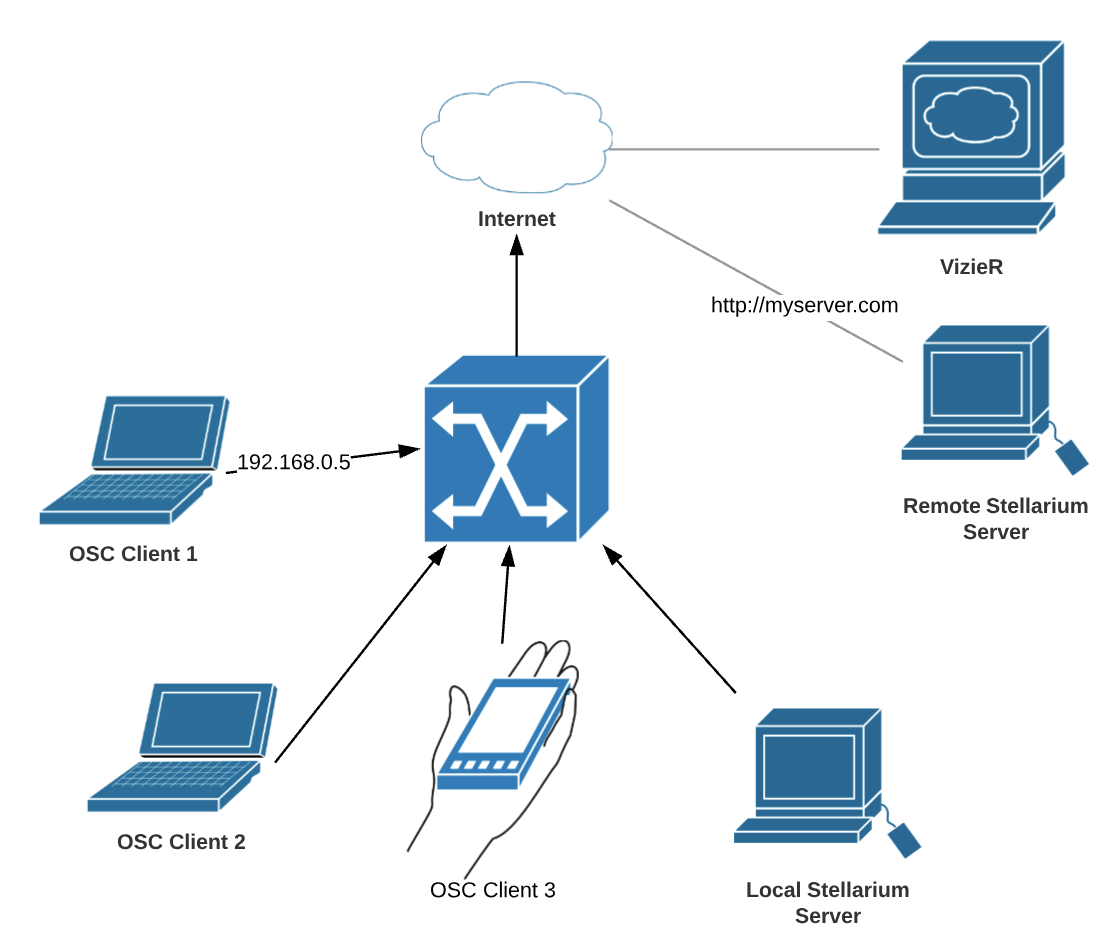
\includegraphics[width=1\columnwidth]{RemoteStellarium}
	\caption{Remote Stellarium and OSC Clients.}
	\label{fig:RemoteStellarium}
\end{figure}
\bigskip

Creating a connection between \textit{OSC Client 1} and \texttt{Remote Stellarium Server} is effected by adding adding the arguments \\\texttt{client=192.168.0.5} and \texttt{stellarium=http://myserver.com} to the command line.
This will cause the Stellar Command module to send OSC messages to ``192.168.0.5" and Stellarium commands to \textit{http://myserver.com} on HTP port 8090\footnote{The default Stellarium Remote Control port is 8090, however, this can be changed inside Stellarium. It is assumed that port forwarding when not using a local area network has been configured to send packages to the correct computer hosting Stellarium}, effectively acting as a proxy between the two.

   \begin{syntax}
	\medskip
	java -jar StellarCommand.jar port=1234 osc=/Stellar  {\char'134}\\client=192.168.0.5 stellarium=http://myserver.com\\
	\medskip
\end{syntax}
\bigskip

\section{Sending Commands to the Stellar Command Module}
You can provide instructions to Stellar Command in order to control Stellarium or to change the amount and type of data you want to receive. For example, you may want the Stellarium display to zoom in closer to a particular area of sky. You would do this by decreasing the field of view.\footnote{Section~\ref{subsec:fieldofview} --
	\emph{\titleref{subsec:fieldofview}} shows how to do this.} Likewise, you may want to reduce the amount of astronomical data you are receiving by adding a filter threshold so VizieR will only receive stars within a certain magnitude range. 

\subsection{Field Of View}\label{subsec:fieldofview}
\chapter{Using Stellar Command as a Java Library} \label{chap:libraryosc}
This chapter details how to use Stellar Command as a library that you call directly from within your programming environment.
If you intend to use Stellar Command as a standalone server application and communicate to it with Open Sound Control Messages through your preferred music package---such as Max MSP, SuperCollider or PD---you can skip back to chapter~\ref{chap:launchosc} --
\emph{\titleref{chap:launchosc}}.
